\documentclass[onecolumn,10pt]{jhwhw}

\usepackage{epsfig} %% for loading postscript figures
\usepackage{amsmath}
\usepackage{graphicx}
\usepackage{caption}
\usepackage{subcaption}
\usepackage{grffile}
\usepackage{pdfpages}
\usepackage{algpseudocode}
\usepackage{wrapfig}
\usepackage{pgfplots}
\usepackage{amsfonts}
\usepackage{booktabs}
\usepackage{siunitx}
\usepackage{commath}
\usepackage{rotating}
\usepackage{url}
\usepackage{multimedia}
\usepackage{hyperref}
\usepackage{mathtools}
\usepackage{dirtytalk}

% Default fixed font does not support bold face
\DeclareFixedFont{\ttb}{T1}{txtt}{bx}{n}{12} % for bold
\DeclareFixedFont{\ttm}{T1}{txtt}{m}{n}{12}  % for normal

% Custom colors
\usepackage{color}
\usepackage{listings}
\usepackage{framed}
\usepackage{caption}
\usepackage{bm}
\captionsetup[lstlisting]{font={small,tt}}

\definecolor{mygreen}{rgb}{0,0.6,0}
\definecolor{mygray}{rgb}{0.5,0.5,0.5}
\definecolor{mymauve}{rgb}{0.58,0,0.82}

\lstset{ %
  backgroundcolor=\color{white},   % choose the background color; you must add \usepackage{color} or \usepackage{xcolor}
  basicstyle=\ttfamily\footnotesize, % the size of the fonts that are used for the code
  breakatwhitespace=false,         % sets if automatic breaks should only happen at whitespace
  breaklines=true,                 % sets automatic line breaking
  captionpos=b,                    % sets the caption-position to bottom
  commentstyle=\color{mygreen},    % comment style
  deletekeywords={...},            % if you want to delete keywords from the given language
  escapeinside={\%*}{*)},          % if you want to add LaTeX within your code
  extendedchars=true,              % lets you use non-ASCII characters; for 8-bits encodings only, does not work with UTF-8
  frame=single,                    % adds a frame around the code
  keepspaces=true,                 % keeps spaces in text, useful for keeping indentation of code (possibly needs columns=flexible)
  columns=flexible,
  keywordstyle=\color{blue},       % keyword style
  language=Python,                 % the language of the code
  morekeywords={*,...},            % if you want to add more keywords to the set
  numbers=left,                    % where to put the line-numbers; possible values are (none, left, right)
  numbersep=5pt,                   % how far the line-numbers are from the code
  numberstyle=\tiny\color{mygray}, % the style that is used for the line-numbers
  rulecolor=\color{black},         % if not set, the frame-color may be changed on line-breaks within not-black text (e.g. comments (green here))
  showspaces=false,                % show spaces everywhere adding particular underscores; it overrides 'showstringspaces'
  showstringspaces=false,          % underline spaces within strings only
  showtabs=false,                  % show tabs within strings adding particular underscores
  stepnumber=1,                    % the step between two line-numbers. If it's 1, each line will be numbered
  stringstyle=\color{mymauve},     % string literal style
  tabsize=4,                       % sets default tabsize to 2 spaces
}

\usepackage{etoolbox}
\renewcommand{\lstlistingname}{Diagram}% Listing -> Algorithm
\patchcmd{\thebibliography}{\chapter*}{\section*}{}{}

\usepackage[utf8]{inputenc}
\usepackage{fourier}
\usepackage{array}
\usepackage{makecell}

% \renewcommand\theadalign{cb}
% \renewcommand\theadfont{\bfseries}
% \renewcommand\theadgape{\Gape[1pt]}
% \renewcommand\cellgape{\Gape[1pt]}

\author{John Karasinski}
\title{HST Rendezvous}

\begin{document}
%\maketitle

\chapter{Introduction}

\begin{figure}[h!]
\begin{center}
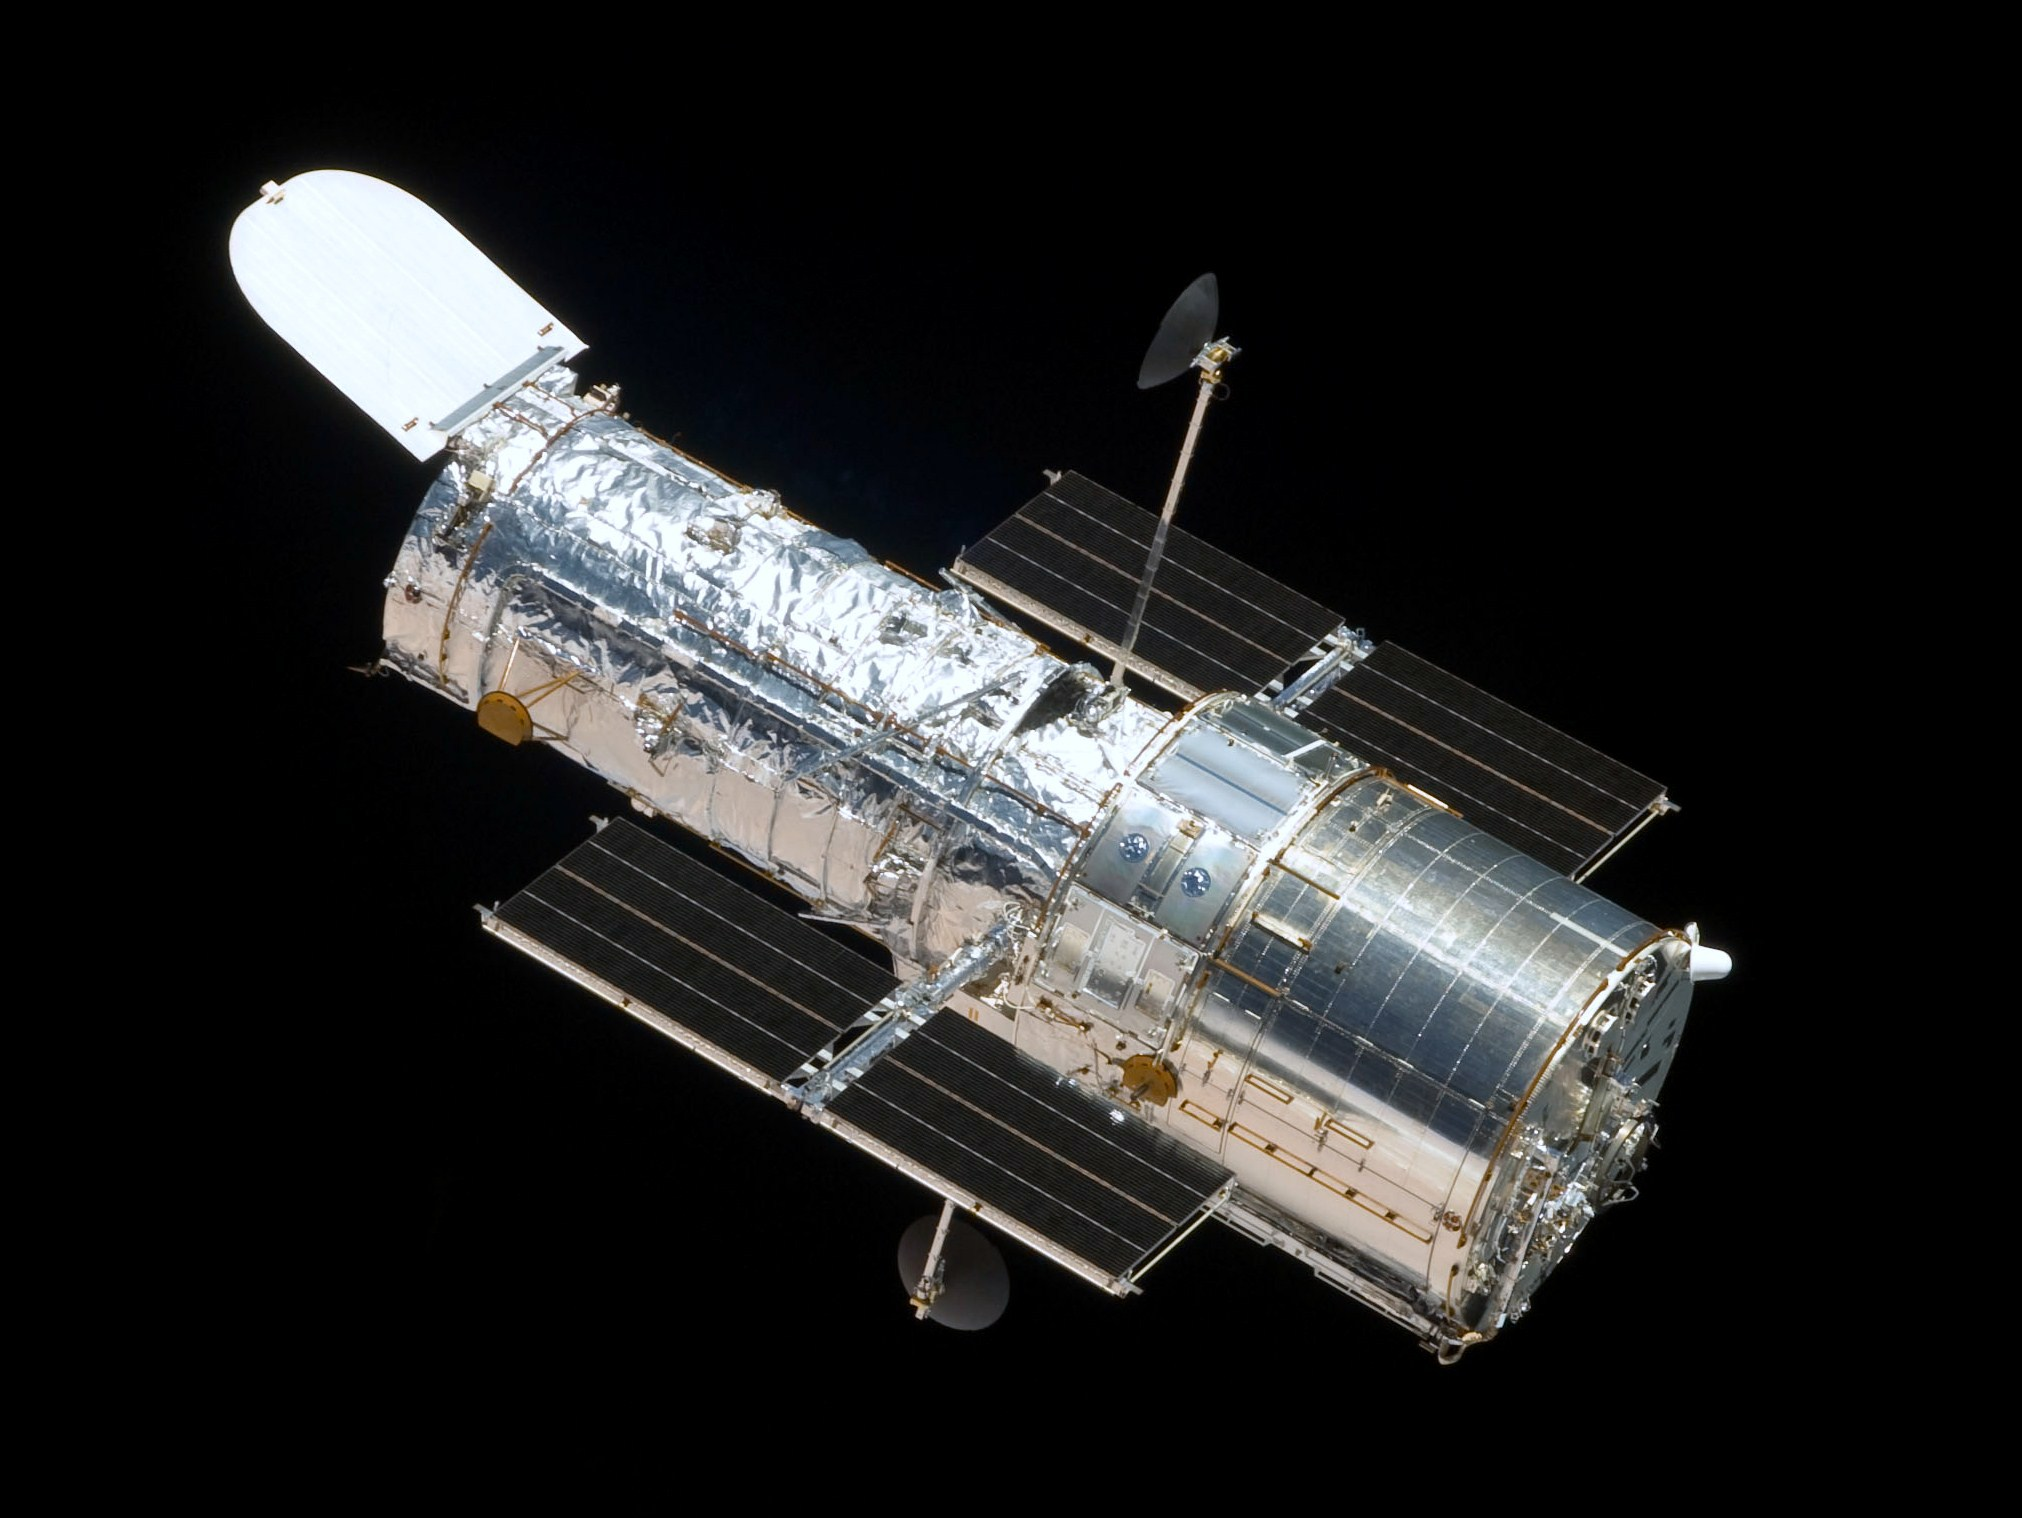
\includegraphics[width=1\textwidth]{imgs/HST-SM4.jpeg}
\caption{The Hubble Space Telescope as seen from the departing Space Shuttle Atlantis, flying Servicing Mission 4 (STS-125), the fifth and final human spaceflight to it.}
\label{fig:density}
\end{center}
\end{figure}

\begin{figure}[h!]
\begin{center}
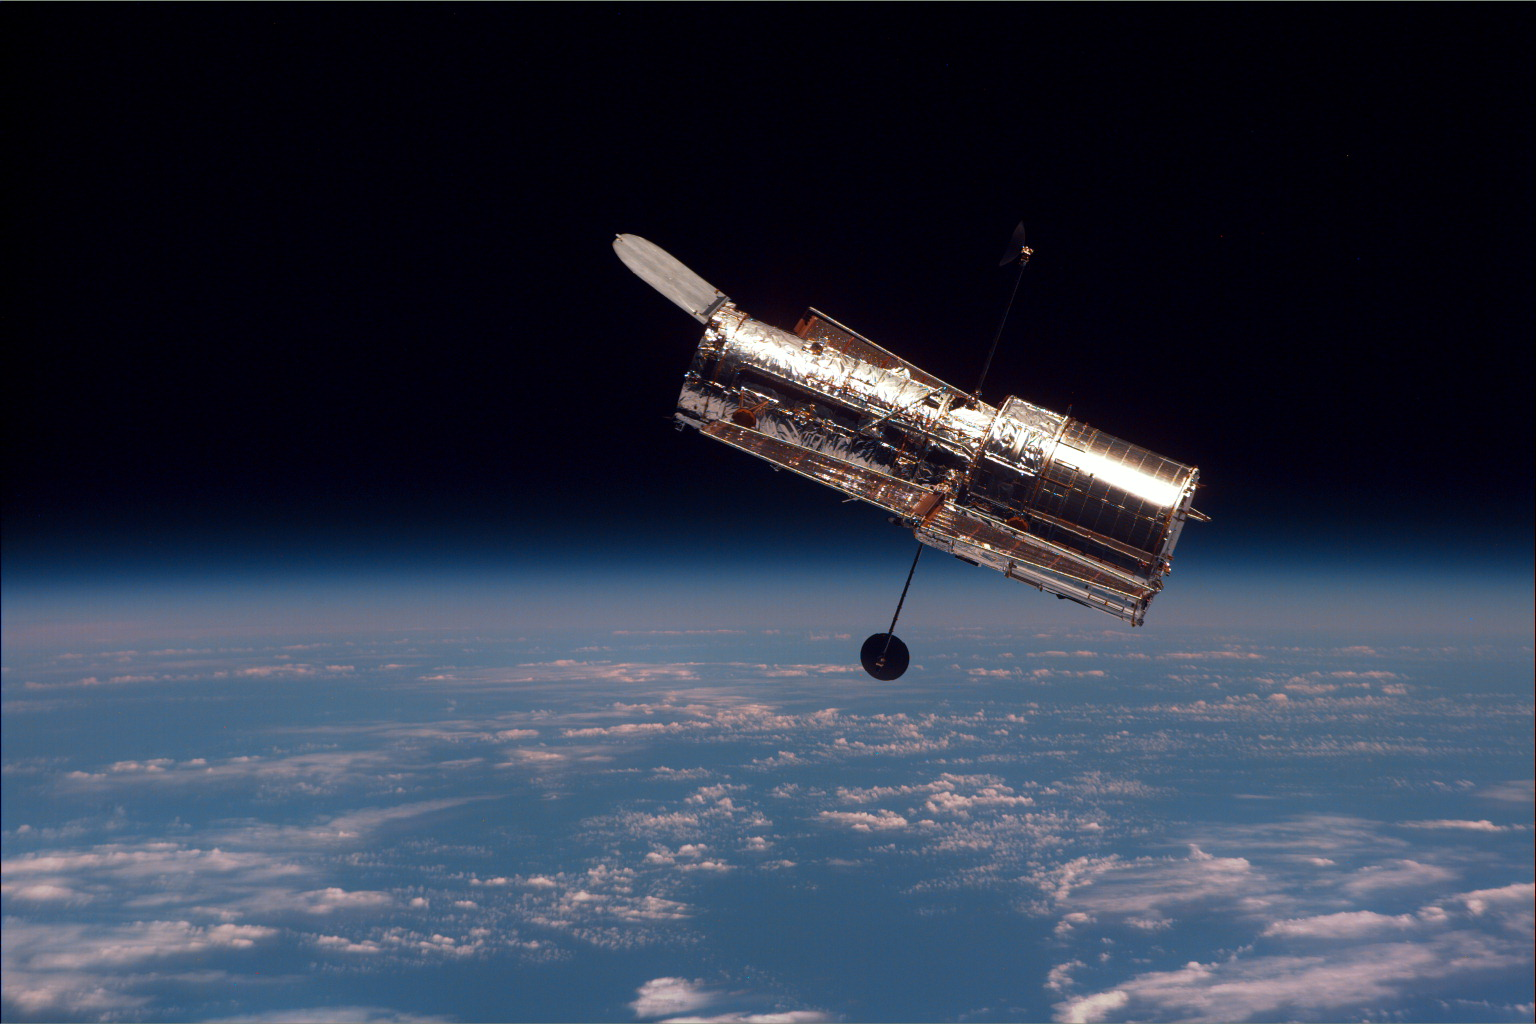
\includegraphics[width=1\textwidth]{imgs/hst.jpg}
\caption{This photograph of NASA's Hubble Space Telescope was taken on the second servicing mission to the observatory in 1997.}
\label{fig:density}
\end{center}
\end{figure}


\section{Stakeholders}

\begin{figure}[t!]
    \centering
    \begin{subfigure}[b]{0.4\textwidth}
        \includegraphics[width=\textwidth]{imgs/xtreme_deep_field.png}
    \end{subfigure}
    ~ %add desired spacing between images, e. g. ~, \quad, \qquad, \hfill etc.
    %(or a blank line to force the subfigure onto a new line)
     \begin{subfigure}[b]{0.4\textwidth}
        \includegraphics[width=\textwidth]{imgs/Pillars_of_creation_2014_HST_WFC3_medium_res.jpg}
    \end{subfigure}
    ~ %add desired spacing between images, e. g. ~, \quad, \qquad, \hfill etc.
      %(or a blank line to force the subfigure onto a new line)
    \begin{subfigure}[b]{0.4\textwidth}
        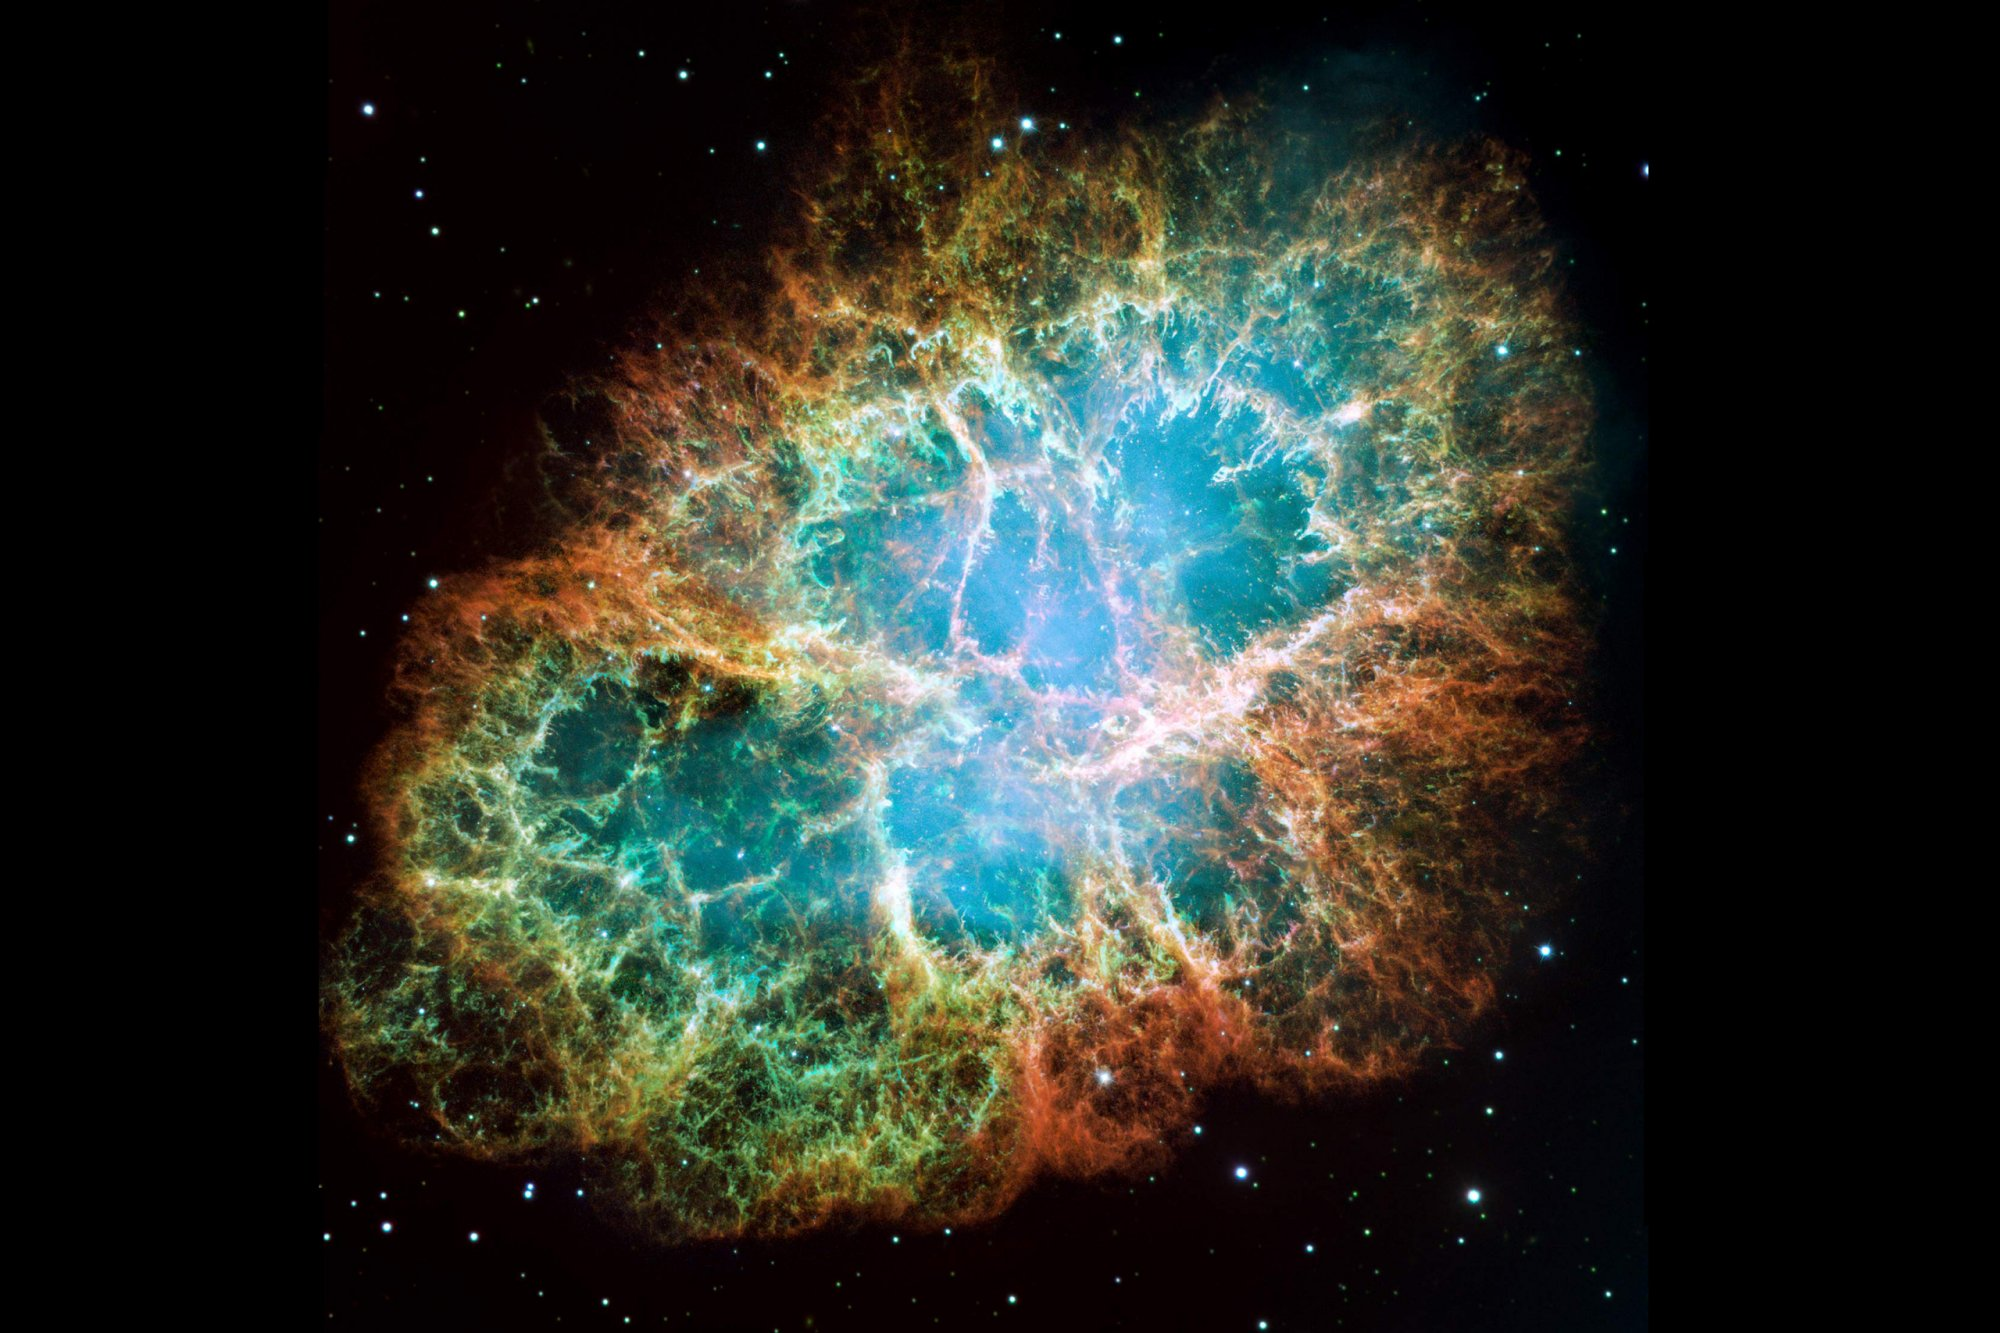
\includegraphics[width=\textwidth]{imgs/crab.jpg}
    \end{subfigure}
    ~ %add desired spacing between images, e. g. ~, \quad, \qquad, \hfill etc.
    %(or a blank line to force the subfigure onto a new line)
    \begin{subfigure}[b]{0.4\textwidth}
        \includegraphics[width=\textwidth]{imgs/M104_ngc4594_sombrero_galaxy_hi-res.jpg}
    \end{subfigure}
    \caption{Hubble has taken many photos of iconic space objects, including the Hubble Extreme Deep Field, Pillars of Creation, the Crab Nebulae, and the Sombrero Galaxy.}
    \label{fig:animals}
\end{figure}

Hubble has a large number of stakeholders. Since it's launch in 1990, the Hubble Space Telescope has acted as one of the most vital research tools for astronomy, and over 9,000 papers based on Hubble data have been published in peer-reviewed journals. Hubble has made a large number of important discoveries, leading to significant changes in how we think about the universe. Among its primary mission targets was to measure distances to Cepheid variable stars more accurately than ever before. Accurate measurement of the Cepheid variable constrains the value of the Hubble constant, the measure of the rate at which the universe is expanding, which has allowed scientists to very accurately calculate the age of the universe.

Hubble has also been extremely successful in generating public relations, both due to its scientific achievements and the wealth of memorable images it has produced. The public is extremely invested in Hubble, both from their large contributions to its construction and operational costs. Aside from Hubble's scientific goals, it also helps fulfill two of NASA's key agency objectives to:
\begin{itemize}
\setlength\itemsep{0em}
\item Improve science literacy by engaging the public in NASA missions and discoveries, and their benefits, through such avenues as public programming, community outreach, mass media, and the Internet.
\item Increase public awareness and understanding of how research and innovations in aerospace technology affect and improve the quality of life.
\end{itemize}

The HST was built by the United States space agency NASA, with contributions from the European Space Agency (ESA). The Space Telescope Science Institute (STScI) selects Hubble's targets and processes the resulting data, while the Goddard Space Flight Center controls the spacecraft~\footnote{"Hubble Essentials". Hubblesite.org. Retrieved March 3, 2016.}. As such, NASA, ESA, STScI, and NASA Goddard are among the chief stakeholders in a robotic reboost mission. Other organizations that have constructed and worked with HST, such as JPL and ITT, would obviously be affected by our interacting with HST. An incomplete list of stakeholders is
\begin{itemize}
\setlength\itemsep{0em}
\item NASA Headquarters (HQ)
\item NASA Goddard Space Flight Center (GSFC)
\item The European Space Agency (ESA)
\item The Space Telescope Science Institute (STScI)
\item The Jet Propulsion Laboratory (JPL)
\item ITT (formerly Kodak)
\item International universities and space agencies
\item The National Reconnaissance Office (NRO)
\item Department of Defense (DoD)
\item Other governmental organizations
\item The public
\end{itemize}

While none of the stakeholders involved in the Hubble project would necessarily mind extending the project for several years, damaging Hubble would be much worse than leaving it in it's current orbit. As such, the primary goal of the HRV is to do no harm to Hubble. The mission can succeed only if we can it can be accomplished within the stakeholders' limits of acceptable risk.

% \section{Concept of Operations}

% \subsection{Communication}
% Chris will write these sections.

% \subsection{What’s ground control doing}
% The Hubble Repair Vehicle (HRV) will act as a primarily automatic vehicle. Despite this, ground control will be in continuous contact with the HRV throughout the lifetime of the mission, and will have the option of delaying or aborting orbital transfers and docking and rendezvous maneuvers. Before each orbital maneuver, ground control will



% After being dropped off from the launch vehicle, HRV will communicate with ground operations. After a brief instrument and spacecraft health check, HRV will receive updated HST state information, and updated orbital rendezvous parameters. Once this information is transferred, HRV will transfer to a higher orbit. HRV will be in contact during the phasing stage of the mission, and will wait at a holding point 15 km behind HST before entering the closing phase.

% \subsection{How’s it going to be used?}


\chapter{Requirements}
\section{Customer Requirements}

The mission of the Hubble Reboost Vehicle (HRV) is to

\say{Reboost HST spacecraft to circular orbit so that useful operation until orbit decay is extended to 5 years beyond the JWST 10/23 launch date, i.e. to 10/28.} \\
\\
Thirteen requirements of the vehicle are taken directly from the Mission Requirements. To this end, the HRV must
\begin{enumerate}
\item Launch on an existing US launcher from Cape Canaveral into the HST orbit
\item Rendezvous and dock with HST
\item Use HST or rebooster ADCS to orient combined spacecraft for reboost
\item Reboost thrust must result in solar array boom deflection of no more than 50 cm
\item Undock from HST and destructively de-orbit into atmosphere
\item Send and receive state-vector, attitude, and system health telemetry to/from HST
\item Send and receive state-vector, attitude, and system health telemetry to/from NASA Mission Control Center (MCC), either directly, or indirectly via HST and or TDRS satellites
\item Be able to recover from one Single Event Upset per hour in the onboard Command and Control Computer
\item No requirement on duration of mission
\item Power and thermal requirements not specified – to be determined by design to meet mission objectives
\item Main body of spacecraft bus must include MMOD shielding
\item ADCS must be able to recover from/override both jet-fail-on, and jet-fail cases during proximity operations without collision of mission failure
\item Loss of communications between rebooster and HST or MCC must not result in collision
\end{enumerate}

\section{Systems Requirements}
\subsection{Rendezvous and Docking}
There is one customer requirement to consider in designing the rendezvous and docking. \say{(b), Rendezvous and dock with HST}.

To address this customer requirement, several system level requirements are set
\begin{enumerate}
\item A rendezvous plan shall be established.
\item A docking plan shall be established.
\item The rendezvous and docking plan shall have sufficient flight heritage.
\item Sufficient sensors shall exist to measure the state of the HRV for both absolute and relative navigation during rendezvous and docking.
\item Sufficient knowledge and control over the vehicle state shall be present in order to meet soft capture mechanism (SCM) docking requirements.
\end{enumerate}

\chapter{Rendezvous and Docking}

\section{Docking}
\subsection{Small Autonomous Satellites}
There have been incredible advancements within the realm of semi-autonomous satellites over the past 20 years. Beginning in 1997, the Autonomous Extravehicular Activity Robotic Camera Sprint (AERCam Sprint) was the first semi-autonomous satellite to demonstrate the use of a free-flying prototype camera aboard the International Space Station (ISS). While operating alongside STS-87 Mission Specialist Winston Scott, the AERCam Sprint flew under the remote-control guidance of Steve Lindsey for approximately 75 minutes, and relayed live television images to Columbia's Mission Control~\cite{Aercam,MiniAercam}. After successfully completing this experiment, researchers and analysts decided to incorporate a higher level of autonomy, and produced a second prototype known as the Mini AERCam in 2000. While this satellite never made it to space, the Mini AERCam underwent multiple tests on an air-bearing table and in an orbital test simulation facility at Johnson Space Center. This newly designed satellite was given automatic position hold, point-to-point maneuvering, and an additional camera to provide an orthogonal view, allowing astronauts to navigate the Mini AERCam with respect to the ISS. Through these multiple additions, researchers expanded the satellite's capability to encompass supervised autonomous and/or remotely piloted operations~\cite{MiniAercam,MiniAercam2}.

In 2006, the first Synchronized Position Hold Engage Reorient Experiment Satellites (SPHERES), a self-contained nanosatellite made by MIT's Space Systems Laboratory, was launched to the ISS and taken to the US Laboratory. Since that time, this semi-autonomous satellite has been joined by two additional SPHERES, making this system the first consistent experimental nanosatellite testbed aboard the ISS. Unlike the AERCam Sprint and the Mini AERCam, SPHERES is a modular satellite where each system is self-contained in individual capsules. This configuration allows SPHERES to easily incorporate system expansions onto specific platforms, such as navigation, without needing to reconfigure the entire craft. Furthermore, its modularity helps researchers efficiently address system failures, making it easier for astronauts to perform on-site repairs. To navigate SPHERES within the ISS, the system utilizes wall-mounted ultrasonic beacons and corresponding ultrasonic receivers attached to the nanosatellite~\cite{SPHERES}. SPHERES emits an infrared flash to determine its location. Once emitted, the satellite waits for the wall-mounted beacons to emit corresponding ultrasonic pulses. After receiving these ultrasonic pulses, the satellite measures its range based on the pulse's time of flight, and can then calculate its relative position, attitude, and angular velocity~\cite{SPHERES,Vertigo1}. This unique navigation system allows SPHERES to emulate a ``pseudo-GPS'' time-of-flight sensing system, and ultimately estimate its position, angular velocity, and attitude without the potential for signal interference and noise -- a challenge that has been previously encountered with GPS systems~\cite{Vertigo1}. Through this autonomous navigation and modular design, the SPHERES testbed has become a versatile platform for developing vision-based navigation, anti-collision, and formation flying algorithms. By allowing research teams to create algorithms that can then be uplinked to the SPHERES test system aboard the ISS, researchers can receive live feedback, and ultimately find the exact areas within their algorithms that need improvement.

\subsubsection{SPHERES VERTIGO}
In 2008 the MIT Space Systems Laboratory began building an upgrade to the SPHERES system, known as the Low Impact Inspection Vehicle (LIIVe), as part of the Visual Estimation and Relative Tracking for Inspection of Generic Objects (VERTIGO) program. Once completed, this upgrade would later be attached to the existing SPHERES system and act as VERTIGO ``goggles,'' allowing SPHERES to perform vision-based navigation experiments in the microgravity environment aboard the ISS. After adjusting these VERTIGO Goggles to suit the space station's environment, the final system was upgraded to include two monochrome stereo cameras, two illuminating LEDs, a 1.2 GHz Via Nano processor, an 802.11n network card, and optics that included a larger aperture lens in a synchronized stereo configuration~~\cite{SPHERES,Vertigo1,Vertigo2,Vertigo3}.

When the modified SPHERES VERTIGO was ready for experimentation, numerous flight algorithms were tested to demonstrate the spacecraft's complete autonomy. After ISS Expedition 34, it was confirmed that SPHERES VERTIGO was capable of autonomously conducting a circular orbit about an uncooperative object, while simultaneously maintaining a constant relative position between SPHERES VERTIGO and the target. This objective was achieved through the primary use of inertial sensors and cameras, and was considered an unprecedented success~\cite{Vertigo2,Vertigo3}.

\subsection{Collision Avoidance and Docking Algorithms}
Since the SPHERES nanosatellite's first microgravity guidance, navigation, and control experiment, there have been three classes of algorithms pertaining to collision avoidance and docking that have emerged: metrology, control, and autonomy~\cite{SPHERES_form}.

The metrology algorithms were implemented using a SPHERES-specific interface, and utilized a series of Extended Kalman Filters to obtain the system's state vector from the sensor outputs. This approach has been typically utilized in position, attitude, and determination systems. Despite many successful implementations, recent literature suggests that the second and third classes have demonstrated greater accuracy in the areas pertaining to collision avoidance and docking~\cite{SPHERES_form}.

The control algorithm class involves both closed-loop controls and path-planning algorithms. One prominent control algorithm that has been frequently tested is the glideslope algorithm. This algorithm is a hybrid between a path-planning and a velocity-control algorithm, where the incoming spacecraft is given commands to slow its velocity as it approaches its target~\cite{SPHERES_form,SPHERES_micro,dist,virt_sim}. The glideslope algorithm was the first autonomous docking algorithm to successfully attach an incoming spacecraft to its tumbling target, and is a relatively simple, yet robust, controller makes this algorithm~\cite{SPHERES_micro}. Another promising algorithm is the ``safe'' trajectory algorithm. This innovative algorithm computes a pre-planned trajectory using the solution from a Mixed-Integer Linear Program, and, using this pre-computed trajectory, is able to optimize fuel and avoid incoming obstacles~\cite{SPHERES_micro}. However, while this algorithm is guaranteed to produce a safe trajectory, its overall complexity requires it to be computed on an external computer. Once the computations have been completed, the final trajectory is transferred to the satellite. This entire computational process creates an approximate nine second delay, and can potentially create a catastrophic outcome if the spacecraft requires an immediate trajectory path to avoid an incoming collision. To remedy this solution, researchers have begun to trade trajectory and fuel optimality for computational time, and can reduce the total computation time to about $0.17$ seconds~\cite{SPHERES_micro}. Lastly, the ``close point of approach'' algorithm has been demonstrated to be both compact and computationally efficient, and has served as a background safety routine for the high school SPHERES Zero Robotics program~\cite{virt_sim}. While all three aforementioned algorithms have accurately performed numerous tests pertaining to collision avoidance and docking, each algorithm is associated with its own specific set of pros and cons. As it currently stands, researchers have yet to find a way to optimize fuel usage, pre-planned trajectories, and computational power, and thus must decide which factors are most important for any given mission~\cite{SPHERES_form,SPHERES_micro,dist,virt_sim}.

Finally, the autonomous algorithm class is used to execute the control class algorithms and determine the current mode of operation~\cite{SPHERES_form}. As a result, the glideslope, ``safe'' trajectory, and ``close point of approach'' algorithms all utilize autonomy to properly perform their respective procedures.

\subsection{Autonomous versus manual docking}
In recent years the small satellite platform has increased in popularity. With the ability to launch multiple small satellites as a secondary payload and the relatively low development cost involved, they are one of the most viable testbeds for new technologies. One great example of this is the class of satellites that adhere to the CubeSat standard~\cite{CubeSat}. CubeSat initiatives have made many projects possible due to the minimal costs required. Although a small size limits their capabilities, higher fidelity projects usually require a larger volume to contain all desired systems. There are several projects that use slightly larger free flyers that have produced unique navigation demonstrations such as AERCam Sprint, Mini-AERCam, and SPHERES ~\cite{Aercam,MiniAercam,SPHERES}. While the Hubble Reboost Vehicle (HRV) is significantly larger than the aforementioned satellites, the rendezvous and docking algorithms developed for these missions can be made just as effective.

These projects make use of an optical sensor to take stereoscopic visual recordings for inspection purposes, and to determine the position and attitude in relation to a target. To do this, the image captured must be used in conjunction with a computer vision algorithm in order to estimate navigational parameters. Using a two color cameras and the full visual light spectrum, a more familiar virtual image is produced. Operators are able to view the subject as if it was in front of them, allowing for quick and informed decision making. This, as among other reasons, has been realized by many research teams and can be seen in many projects such as SPHERES VERTIGO and the aforementioned AERCam projects~\cite{Aercam,MiniAercam,Vertigo1}.

Most current docking procedures utilize a laser range finder for determining distance. Laser range finders have flight heritage and have moderate accuracy~\cite{Docking}. Simple fiducial markers can be used to increase the performance of range finders, and multiple markers can allow rangefinders to triangulate a relative position. Markers for visual navigation systems, however, can vary in complexity. Marker distribution and marker shape can allow a computer vision system to gather a large amount of data with a single image, whereas a laser rangefinder must take multiple measurements. This system was originally developed for manual docking operations, but it also provides visual information to allow more accurate computer vision position measurements.

In ground-based scenarios, the only drift from the intended rendezvous trajectory is contributed to error or disturbances, but in this situation there is also drift due to the inspector and the target occupying different orbits. Even with a perfect initial trajectory and planning, corrections are required. The navigation scheme must be as efficient as possible as course corrections are unavoidable.

The great distances involved in satellite operation, coupled with an inherent delay involved with routing signals to a ground station, however, make human operation of the HRV infeasible. A one-way time delay of a few seconds from a satellite to the ground-based operator, with the addition of just one second of human operator delay, with the additional delay of a few seconds back from the ground-based operator to the satellite result of time delays greater than 5-10 seconds, at which point it is too late to make corrections. An automated system, based on the navigation schemes outlined above, has a much greater chance for success. Such a system can make nearly instantaneous decisions, and can execute them before a human operator has time to identify the situation. Coupling an automated docking procedure with a human backup to abort gives the best of both scenarios. The automated docking system can handle the lower level task of docking, and the human operator is present to abort the docking attempt if unexpected errors occur.

\section{Rendezvous}

\subsection{How will we rendezvous, and how long does rendezvous take?}
\begin{figure}[t!]
\begin{center}
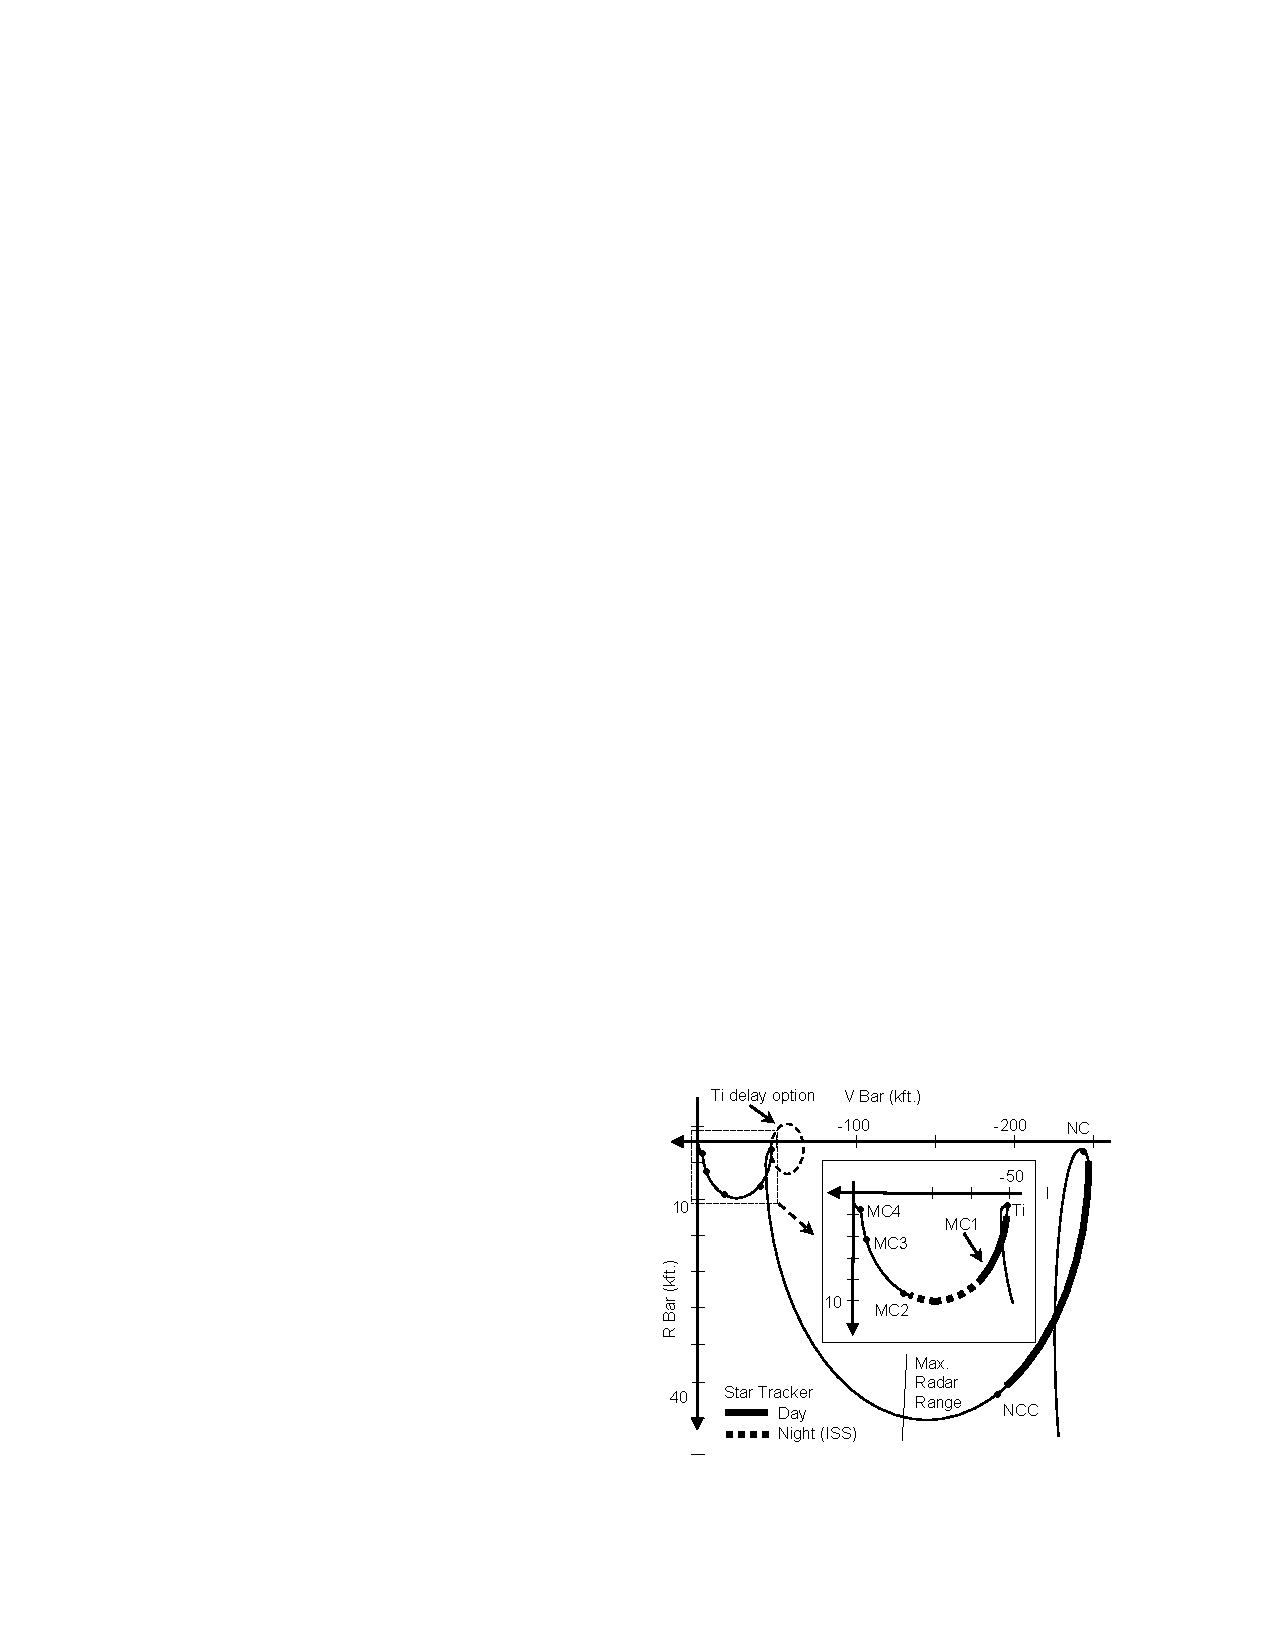
\includegraphics[width=.5\textwidth]{imgs/orbt.pdf}
\caption{Optimized R-Bar Targeted Rendezvous (ORBT) relative navigation rendezvous diagram.}
% \label{fig:density}
\end{center}
\end{figure}

Current orbital decay predictions place the Hubble Space Telescope (HST) at a nearly circular, 528 km altitude orbit during our proposed launch date of January 2020. After launch, we will enter a 200 km, in-plane parking orbit, then enter a 500 km phasing orbit. From our phasing orbit, we will perform a homing maneuver bring us to a holding point 15 km behind HST. When relative navigation sensors have acquired HST, we will perform a closing maneuver to bring us to 500 m below HST, after which an R-bar approach will be used to bring us to dock.

For the R-bar approach, our vehicle move up towards HST along its radial vector. Our vehicle will fire thrusters radially to close towards HST, and use small burns in the orbital velocity direction to negate the effects of orbital mechanics. If the R-bar is stopped at any point (in case of loss of communication or thruster failure, for instance), our vehicle will naturally move away from HST. If, at any point in the docking, communication is lost, the HRV will automatically return to a holding point behind HST.

This approach has been adapted from the from the Space Shuttle's Optimized R-Bar Targeted Rendezvous (ORBT) profile~\footnote{Goodman, John L. ``History of Space Shuttle Rendezvous.'' (2011).}. ORBT was developed to optimally set up initial conditions for a low energy coast up the +R-bar. This profile was used from 1997 to the end of Space Shuttle program in 2011, lending more than a decade of operational flight heritage.

\subsection{At what stage of the rendezvous are sensors active? Can we recover from a single sensor failure at each stage?}
\begin{table}[tb]
\begin{center}
\begin{tabular}{c c c c}
\toprule
Sensor & \# On-board & Upper Range & Lower Range \\
\midrule
Radar        & 2 & 100s of km & 100s of m  \\
LIDAR        & 2 & 10s of km & 2m  \\
Camera       & 2 & 100s of m & contact  \\
GPS          & 2 & - & -  \\
\bottomrule
\end{tabular}
\end{center}
\caption{Relative and absolute navigation sensors onboard the HRV.}
% \label{properties}
\end{table}

\begin{table}[tb]
\begin{center}
\begin{tabular}{c c c c}
\toprule
Sensor & \# On-board & Performance \\
\midrule
Horizon Sensor & 2 & 0.25 deg \\
Sun Sensor     & 1 & 0.01 deg \\
Startracker    & 2 & 0.005 deg \\
IMU            & 2 & 0.003 deg/hr \\
\bottomrule
\end{tabular}
\end{center}
\caption{Attitude measurement sensors onboard the HRV.}
% \label{properties}
\end{table}

The most likely cause of failure for our spacecraft is a loss of attitude measurement. When the spacecraft is phasing with HST, its sources of attitude measurement are startrackers, a sun sensor, horizon sensors, and IMUs. Without frequent updates from the other attitude sensors, however, the IMUs experience drift and quickly become useless. Once the spacecraft comes within a few 10s of km of HST, however, radar and LIDAR can also be used calculate relative attitude. During final approach, the last few 100 m, stereo cameras can calculate sufficient pose estimation for docking.

There are at least two sensors available at all times for both attitude and navigation during all parts of the mission. During all phases of the mission, except for final rendezvous and docking, GPS navigation is sufficient to navigate. Once we begin the final stages of rendezvous and docking, there are three types of relative navigation sensors available. Two redundant radar sensors can be used to initially make relative navigations, and we can transition to LIDAR and optical measurements for the final 100s of meters. Horizon and sun sensors, and star trackers can be used for absolute attitude measurement for the early stages of the mission, and LIDAR and optical measurements can be used for relative pose navigation during the final stages of docking.

\begin{table}[tb]
\begin{center}
\begin{tabular}{c c c c}
\toprule
Sensor & Displacement Error & Rate Error \\
\midrule
Lateral   & 11.4 cm & 1.3 cm/s \\
Range     & 20.3 cm & 5.1 cm/s \\
Roll      & 4 deg   & 1 deg/s \\
Pitch/Yaw & 4 deg   & 0.25 deg/s \\
\bottomrule
\end{tabular}
\end{center}
\caption{}
% \label{properties}
\end{table}


\subsection{How long can we stay at each part of the orbit?}

If sufficient time has passed without contact with ground control, the HRV should automatically perform a deorbit burn. If additional failures, such a major electrical issue, prevent the HRV from deorbiting, there is a possibility of remaining in orbit for much longer than the intended mission duration.

Various orbital perturbations such as gravity gradients, solar pressure, magnetic field interactions, and atmospheric drag can decrease the altitude of the orbit. Of these factors, the largest for low Earth orbit is drag, which increases exponentially as the spacecraft lowers altitude. The acceleration due to drag is
\begin{align*}
D &= \dfrac{1}{2} \rho v^2 A C_d
\end{align*}
in the direction opposite of the spacecraft's velocity. Here $\rho$ is the density of the atmosphere, $A$ is the area exposed to the atmosphere, and $C_D \approx 2.2$ is the coefficient of drag. The solar radio flux can also change dramatically with the solar cycles, and has strong affects on the atmosphere. A program was developed under the assumptions of constant satellite mass, LVLH attitude, and $C_D$. $\rho$ is modeled as an exponential factor based on altitude.

There are three main circular orbits that the mission will take place in: 200km orbit, 536km orbit, and a 616km orbit. As the satellite boosts itself (and Hubble) to higher, it expends fuel, which means that our satellite will always have a lower mass at higher orbits. The results and input parameters of the orbit lifetime analysis are listed in Table~\ref{altitude_table}. Satellites will remain in orbit longer at higher altitudes, where the atmospheric density is lowest. As such, the longest orbital lifetimes are at highest orbit, and the shortest lifetimes are at low altitudes. If satellite communication is not established within the first three days, the HRV will destructively re-enter the atmosphere.

% \begin{table}[tb]
% \begin{center}
% \begin{tabular}{rrrrr}
% \toprule
% Altitude & 200km & 536km & 616km \\
% \midrule
% $m$ & 996 kg & 881 kg & 637 kg \\
% $t$ & 2.9 days & 99.5 years & 380 years \\
% \bottomrule
% \end{tabular}
% \end{center}
% \caption{$C_D$=2.2, $A=4$m$^2$}
% \label{altitude_table}
% \end{table}

\begin{table}[tb]
\begin{center}
\begin{tabular}{lrrrrr}
\toprule
Mass (kg) &           600  &           700  &           800  &           900  &           1000 \\
Altitude (km)     &                &                &                &                &                \\
\midrule
100.0 &       0.3 &       0.3 &       0.4 &       0.4 &       0.4 \\
237.5 &      12.4 &      14.4 &      16.5 &      18.5 &      20.5 \\
375.0 &     544.7 &     635.4 &     726.1 &     816.8 &     907.5 \\
512.5 &   15073.3 &   17585.4 &   20097.5 &   22609.6 &   25121.7 \\
650.0 &  257994.8 &  300993.8 &  343992.8 &  386991.8 &  429990.8 \\
\bottomrule
\end{tabular}
\end{center}
\caption{Time to deorbit, in days with $C_D$=2.2, $A=4$m$^2$.}
\label{altitude_table}
\end{table}

\lstinputlisting[caption=Orbital decay python script.]{decay.py}

\chapter{Historical Data}

% \begin{table}[h]
% \begin{center}
% \begin{tabular}{|c |c |c |c |c|}
% % \toprule
% \hline
% Maneuver & Time, MET & System & $\Delta$V, ft/sec & Duration, sec \\
% % \midrule
% \hline
% NC-1  & 00:05:27:28.9 & OMS (Both) & 98.0 & 59.2 \\ \hline
% NSR   & 01:03:43:59.7 & OMS (Both) & 49.8  & 30 \\ \hline
% NC-2  & 01:04:17:14.3 & OMS (Left) & 14.1 & 17.1 \\ \hline
% NC-3  & 01:17:55:30.1 & OMS (Right) & 12.1 & 14.8 \\ \hline
% % \bottomrule
% \end{tabular}
% \end{center}
% \caption{STS-61. The HST was grappled at 01:23:19:56 and berthed at 01:23:57:30.}
% % \label{properties}
% \end{table}

% % \begin{table}[h]
% % \begin{center}
% % \begin{tabular}{|c |c |c |c |c|}
% % % \toprule
% % \hline
% % Maneuver & Time, MET & System & $\Delta$V, ft/sec & Duration, sec \\
% % % \midrule
% % \hline
% % Reboost 1  & 06:16:59 & RCS Vernier (?) & - & 61 \\ \hline
% % % \bottomrule
% % \end{tabular}
% % \end{center}
% % \caption{STS-61. The HST was grappled at 01:23:28 and berthed at 2:00:10.}
% % % \label{properties}
% % \end{table}

% \begin{table}[h]
% \begin{center}
% \begin{tabular}{|c |c |c |c |c|}
% % \toprule
% \hline
% Maneuver & Time, MET & System & $\Delta$V, ft/sec & Duration, sec \\
% % \midrule
% \hline
% NSR   & 01:03:36:21.9  & OMS         & 96  & 56.2 \\ \hline
% NC-2  & 01:05:02:00    & RCS Primary & 3.1 & 13.0 \\ \hline
% NH    & 01:17:06:04.9  & OMS         & 12  & 8.0  \\ \hline
% NC-3  & 01:17:53:00    & RCS Primary & 3.4 & 14.0 \\ \hline
% NPC-2 & 01:19:00:24    & RCS Primary & 0.5 & 2.0  \\ \hline
% NCC   & 01:20:07:46    & RCS Primary & 1.1 & 1.1  \\ \hline
% TI    & 01:21:07:52    & RCS Primary & 2.8 & 12.0 \\ \hline
% MC-1  & 01:21:34:16    & RCS Primary & 0.4 & 2.0  \\ \hline
% MC-2  & 01:22:02:40    & RCS Primary & 1.5 & 6.0  \\ \hline
% MC-3  & 01:22:12:40    & RCS Primary & 0.9 & 3.0  \\ \hline
% MC-4  & 01:22:22:40    & RCS Vernier & 0.2 & 1.0  \\ \hline
% % \bottomrule
% \end{tabular}
% \end{center}
% \caption{STS-82. The HST was grappled at 01:23:28 and berthed at 2:00:10.}
% % \label{properties}
% \end{table}

% % \begin{table}[h]
% % \begin{center}
% % \begin{tabular}{|c |c |c |c |c|}
% % % \toprule
% % \hline
% % Maneuver & Time, MET & System & $\Delta$V, ft/sec & Duration, min:sec \\
% % % \midrule
% % \hline
% % Reboost 1 & 04:01:09:28 & RCS Vernier & 6.6  & 20:41.9 \\ \hline
% % Reboost 1A$_a$ & 04:06:07:04 & RCS Vernier & 3.3  & 10:12.6 \\ \hline
% % Reboost 2 & 5:01:15:03 & RCS Vernier & 6.5  & 19:46.9 \\ \hline
% % Reboost 3 & 07:01:33:00 & RCS Vernier & 10.4 & 31:53.5 \\ \hline
% % % \bottomrule
% % \end{tabular}
% % \end{center}
% % \caption{STS-82. a - Manuever required for space debris avoidance. The four reboost maneuvers raised the HST orbit an average of 8 nmi.}
% % % \label{properties}
% % \end{table}

\begin{table}[h]
\begin{center}
\begin{tabular}{|c |c |c |c |c|}
% \toprule
\hline
Maneuver & Time, MET & System & $\Delta$V, ft/sec & Duration, sec \\
% \midrule
\hline
NC-1 Trim & 01:03:42:23    & RCS Primary & 0.06 & 0.44   \\ \hline
NC-2      & 01:04:36:49    & RCS Primary & 7.4  & 31     \\ \hline
NSR Trim  & 01:17:36:55.1  & RCS Primary & 0.2  & 0.24   \\ \hline
NCC       & 01:20:38:00    & RCS Primary & 0.3  & 1.0    \\ \hline
TI        & 01:21:36:06    & RCS Primary & 4.1  & 8.7    \\ \hline
MC-1      & 01:21:58:06    & RCS Primary & 0.3  & 0.5    \\ \hline
MC-2      & 01:22:32:58    & RCS Primary & 0.9  & 2.9    \\ \hline
MC-3      & 01:22:49:58    & RCS Primary & 0.4  & 1.0    \\ \hline
MC-4      & 01:22:59:58    & RCS Vernier & 1.8  & 7.2    \\ \hline
% \bottomrule
\end{tabular}
\end{center}
\caption{STS-103. The HST was grappled at 01:23:44:01 and berthed at 2:00:52.}
% \label{properties}
\end{table}


\begin{table}[h]
\begin{center}
\begin{tabular}{|c |c |c |c |c|}
% \toprule
\hline
Maneuver & Time, MET & System & $\Delta$V, ft/sec & Duration, sec \\
% \midrule
\hline
NC2  & 000:17:50:50.5 & -X RCS & 4.5 & 19.7 \\ \hline
NC3  & 01:02:55:32    & Multi-axis RCS & 3.1 & 12.6 \\ \hline
NC4  & 01:17:47:01    & Multi-axis RCS & 4.8 & 20.4 \\ \hline
NCC  & 01:18:38:57    & Multi-axis RCS & 1.3 & 5.5 \\ \hline
MC-1 & 01:19:59:04    & Multi-axis RCS & 0.8 & 3.2 \\ \hline
MC-2 & 01:20:34:27    & Multi-axis RCS & 0.4 & 1.79 \\ \hline
MC-3 & 01:20:34:27    & +X RCS & 1.9 & 8.1 \\ \hline
MC-4 & 01:21:01:28    & Multi-axis RCS & 1.9 & 8.1 \\ \hline
% \bottomrule
\end{tabular}
\end{center}
\caption{STS-109. The HST was captured at 001:21:09:19.}
% \label{properties}
\end{table}

% \begin{table}[h]
% \begin{center}
% \begin{tabular}{|c |c |c |c |c|}
% % \toprule
% \hline
% Maneuver & Time, MET & System & $\Delta$V, ft/sec & Duration, min:sec \\
% % \midrule
% \hline
% Reboost 1 & 07:05:56:01.8 & RCS Vernier (?) & 11.8  & 36:00 \\ \hline
% % \bottomrule
% \end{tabular}
% \end{center}
% \caption{STS-109. The reboost maneuver raised the HST orbit an average of 3.6 nmi.}
% % \label{properties}
% \end{table}

\begin{table}[h]
\begin{center}
\begin{tabular}{|c |c |c |c |c|}
% \toprule
\hline
Maneuver & Time, GMT & System & $\Delta$V, ft/sec & Duration, sec \\
% \midrule
\hline
NC 1 & 131/21:49:54.65 & RCS & 19.5 & 90.88   \\ \hline
NCC  & 133/13:41:50    & RCS &  1.6 & 7.0     \\ \hline
MC 3 & 133/15:53:26.3  & RCS &  0.9 & 0.2     \\ \hline
MC 4 & 133/16:03:26.5  & RCS &  2.1 & 8.9     \\ \hline
% \bottomrule
\end{tabular}
\end{center}
\caption{STS-125. The HST was captured at 133/17:30:52.}
% \label{properties}
\end{table}

% \nocite{*}
\bibliographystyle{IEEETran}
\bibliography{bib}{}

\end{document}

